%!TEX root=../document.tex

\section{How did it all start?}

Countries around the European Union have not been ideal places to live recently. The countries, that are included in this crisis, are mostly from the Mideast and Africa. All together nine civil wars are going on in these regions. This is why there are so many refugees fleeing for their lives. About 11 million people of the population of Syria have been forced to leave their homes, with over four million refugees from other countries.

\section{Reasons}

Civil wars are not the only reason for this crisis. Weak economies causing the population to leave their places and find better ones, with more stable political and social environment. And if that is not enough, an organisation called ISIS (Islamic State of Iraq and Syria) developed through this time. They use the downsides of these developing countries for their advantage. Recruiting young people to fight on their side for their ideology.

\section{The civil war in Syria}

Syria has been going through a brutal civil war for four years now. In 2011, Syria many government protests broke out.
Back then the current president with the name ''Bashar al-Assad'' did not appreciate these and responded with a massive killing spree, killing those who disagreed with him. This prompted resistors to build groups, and arm them with lethal weapons against him. This developed into a full-blown civil war, with at least a thousand of rebel groups with different mindsets.

Both sides leaked information, about having chemical weapons in their property. In August 2013, images surfaced that appeared to show a massive chemical attack on civilians in Syria. The United States blamed Assad and Assad blamed the rebels.
For a time it looked like the US was on the brink of military intervention in Syria. Then the UN (United Nations) and Assad cut a deal, to destroy all chemical weapons. The talk of intervention cooled off, for a while.

One of the most famous rebel group named ISIS has been indirectly helpful to Assad, since he has been more focused on defeating other organisations, that set their goal to take him down, ISIS was fighting other rebel groups instead of him.
This renderd ISIS the opportunity to take more land under their control and become even more powerful. So powerful that last September, the US started for the first time with airstrikes.

\section{How are they getting to the EU?}
Most of the people are paying smugglers for spots on overcrowded fishing boats or inflatable dinghies (little boats), trains or buses. Thousands of them have died while trying to make it to the EU.

One big disaster happended on the 26th of August 2015. 71 refugees died inside a reefer, which was on the way from Hungary towards Austria. It was found next to a village called ''Pandorf'' on a highway without a driver. As the police arrived, decay liquid was already dropping out of the truck. The responsible organization for this disaster is a hungarian smuggler group.

\section{EU on the edge of its breakdown}
Allthough Germany has had the most asylum applications in 2015, Hungary had the highest in proportion to its population, despite having closed its border with Croatia in an attempt to stop the flow in October. Nearly 1,800 refugees per 100,000 of Hungary´s local population claimed asylum in 2015.

Sweden followed close behind with 1,667 per 100,000.

The figure for Germany was 587 and for the UK it was 60 applications for every 100,000 residents. The EU average was 260.

\begin{figure}[!h]
	\begin{center}
		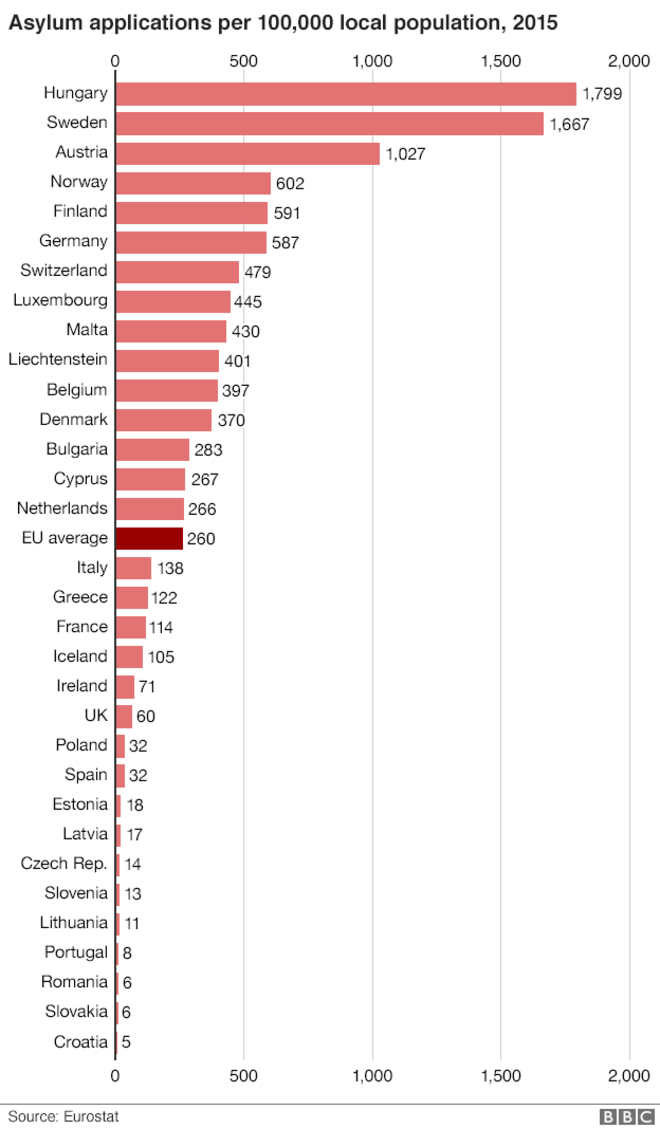
\includegraphics[width=0.5\linewidth]{images/asylums_per_100k}
		\caption{Asylum applications per 100,000 local population}
		\label{broker}
	\end{center}
\end{figure}

\subsection{Response from Europe}
The European Union decided to evenly redistribute about 160,000 refugees EU-wide particulary from countries where the majority of migrants have been arriving. Affected countries are Italy, Greece. The following chart will describe the relocation-plan of the Union.

\begin{figure}[!h]
	\begin{center}
		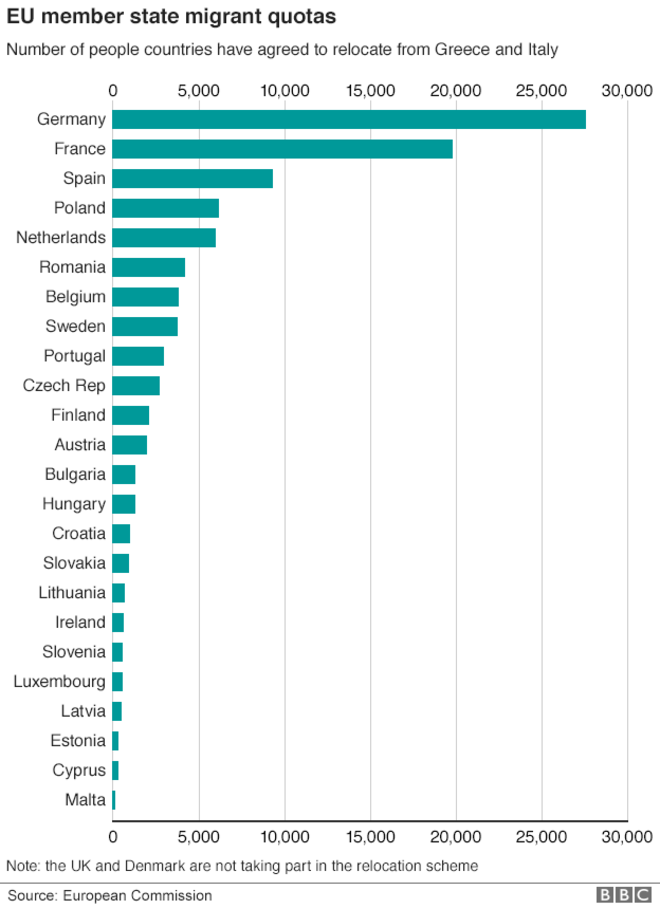
\includegraphics[width=0.5\linewidth]{images/asylums_redistribution}
		\caption{Number of people countries have agreed to relocate from Greece and Italy}
		\label{broker}
	\end{center}
\end{figure}
\newpage
\section{Has the refugee crisis uncovered the downsides of \mbox{globalization}?}

According to information gathered in 2013, there are 232 million of migrants. Migrant waves are mostly heading towards USA, Russia and Europe. These are mainly economic migrants. Others are forced migrants or refugees affected by wars or deconstruction of countries due to export of democracy and search for vast oil fields in the Middle East and all over the world. Refugee crisis in Europe encompasses economic, forced, illegal migrants and refugees. It is a heterogenous group on the move or a new Migration Period in the age of the second modernity. They are being currently used as a powerful biopolitical and potential economic weapon in conquering space and transforming cultural identities in the long run, as it is the case in Europe. Europe is being confronted with an unexpected refugee crisis. The case of refugee crisis, which exemplifies and shows the ugly side of globalization, has made Europe look like a bad tempered instrument of imaginary power in evident postmodern condition.

Multinational corporations are accused of social injustice, unfair working conditions, as well as lack of concern for environment, mismanagement of natural resources, and ecological damage. This causes many people to leave and find better places to live, like mentioned before.

\section{Conclusion}
Refugees have been accepted

